\documentclass[11pt,compress,t,notes=noshow, aspectratio=169, xcolor=table]{beamer}

\usepackage{../../style/lmu-lecture}
% Defines macros and environments
 
%\title{iML: Post-hoc Methods for Neural Networks}
%\subtitle{Motivation}

\title{Interpretable Machine Learning}
\date{}

\begin{document}
%	\maketitle
	\graphicspath{ {./figure/} }

\newcommand{\titlefigure}{figure/iml-grad-vis}
\newcommand{\learninggoals}{
\item Interpretability in neural networks
\item Landscape of interpretability
\item The difference between feature visualization and feature attributions}

\lecturechapter{Post-hoc Methods for Neural Networks}
\lecture{Motivation}
	
\begin{frame}[c]{Neural Networks as Complex ML models}
	\pause
	\begin{itemize}
		\item Neural networks are over parameterised
		\begin{itemize}
			\item Vision models and Language models routinely have > millions of params
			\item Sometimes \#parameters > \#input instances
			\item Which and how do the features, parameters, training instances contribute towards
				  the final decision ?
		\end{itemize}
	\end{itemize}
	\pause

	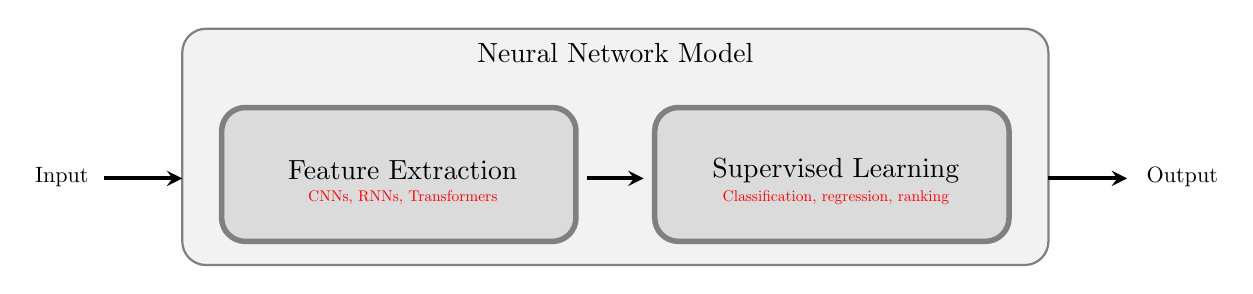
\begin{tikzpicture}
		\hfill	\filldraw[color=gray, fill=gray!10, rounded corners= 3mm, thick]  (-1,0) rectangle (10,-3); 
		\node at (4.5, -0.3) {Neural Network Model}; 
		\filldraw[color=gray, fill= gray!28, rounded corners= 3mm, line width= 0.7mm] (-0.5, -1) rectangle (4, 					-2.7);
		\node  at (1.8, -1.8) {Feature Extraction};
		\node [color=red, scale=0.56] at (1.8, -2.15) {CNNs, RNNs, Transformers};
		\draw [-stealth,line width = .5mm, scale= 2] (-1, -0.95) -- (-0.50, -0.95);
		\node [scale= 0.8] at (-2.53, -1.88) {Input};
		\draw [-stealth,line width = .5mm, scale= 2] (5, -0.95) -- (5.50, -0.95);
		\draw [-stealth,line width = .5mm, scale= 2] (2.07, -0.95) -- (2.43, -0.95);
		\filldraw[color=gray, fill= gray!28, rounded corners= 3mm, line width= 0.7mm] (5, -1) rectangle (9.5, -2.7);
		\node [scale= 0.8] at (11.7, -1.88) {Output};
		\node [color=red, scale=0.56] at (7.3, -2.15) {Classification, regression, ranking};
		\node at (7.3, -1.8) {Supervised Learning};
\end{tikzpicture}
\end{frame}


\begin{frame}{Neural Networks as Complex ML models}
	\begin{itemize}
		\item Neural networks are compositional and non-linear systems
		\begin{itemize}
			\item The success of neural networks is due to their depth
			\begin{itemize}
				\item Depth results in compositional behaviour
			\end{itemize}
			\item Non-linearity between layers helps capture non-linear relationships
		\end{itemize}
		\bigskip
		
		\item Depth and non-linearity leads to lack of interpretability
	\end{itemize}

    \hfill
    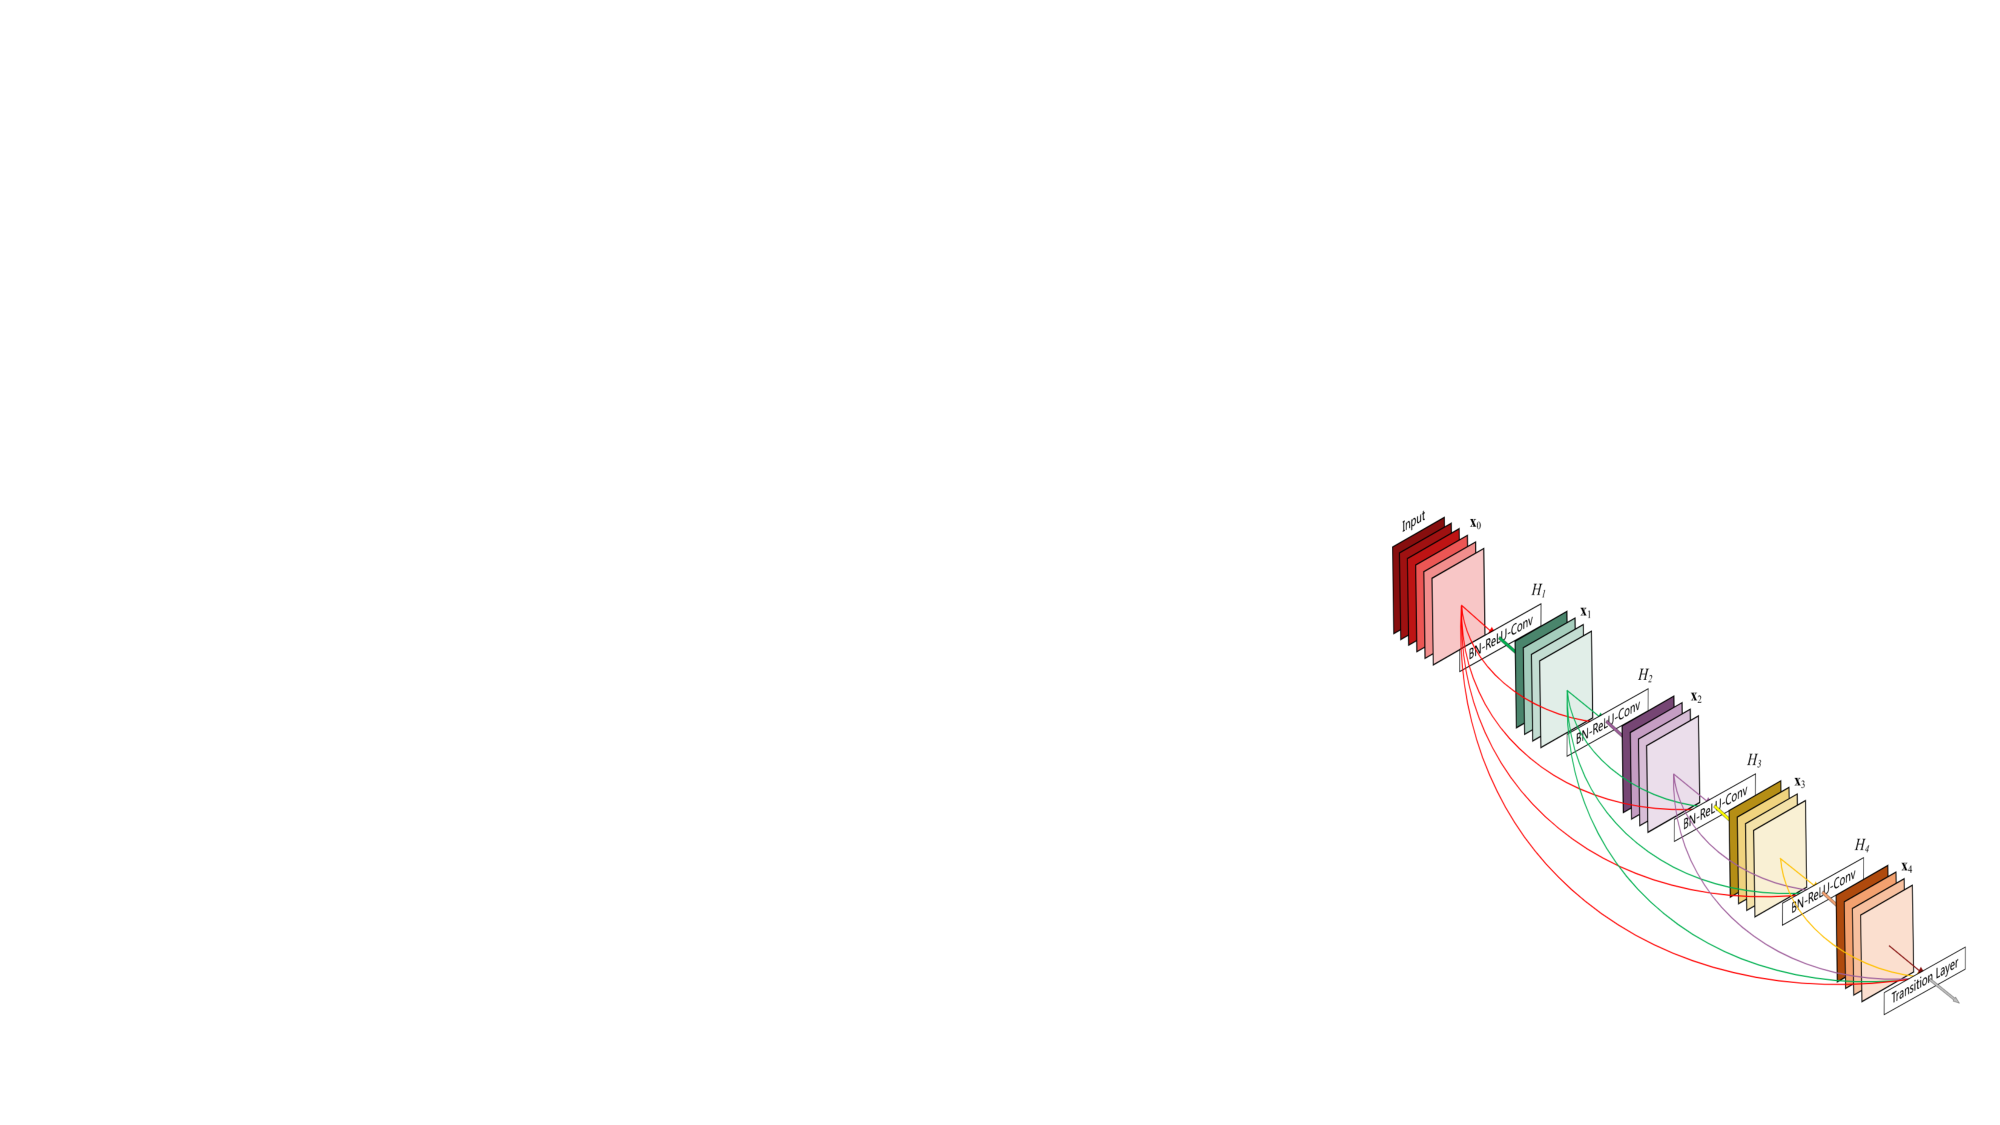
\includegraphics[width=0.3\linewidth]{img116}

\end{frame}

\begin{frame}[c]{Model-specific interpretability}
	\begin{itemize}
		\item What types of neural models are out there ?
		\begin{itemize}
			\item For vision: Convolutional Neural Nets
			\item For language, speech: Recurrent Neural Nets, Transformer Models
			\item For recommendation systems, ranking: Factorization-based Models, Embeddings
models
		\end{itemize}
		\item Each of the domains have their challenges and have developed specific approaches for
interpretability
		\begin{itemize}
			\item We will focus on first principles that can be applied to most models
			\item We will discuss adaptations to each data modality as and when required
		\end{itemize}
	\end{itemize}
	
\end{frame}

%\begin{frame}[c]{Interpretability landscape in Neural Networks}
%     \begin{tikzpicture}
% 	\filldraw[color=gray, fill=gray!28, rounded corners= 3mm, very thick]  (-1,0) rectangle (6,-1); 
% 	\node at (2.5, -0.5) {Interpretability}; 
% 	\filldraw[color=gray, fill= gray!28, rounded corners= 3mm, very thick] (-2.8, -3) rectangle (0, -4.0);
% 	\node  [scale=.7] at (-1.4, -3.4) {Interpretability by 
% };
% 	\node  [scale=.7] at (-1.5, -3.7) {desgin
% };
% 	\node [color=red, scale=0.56] at (2.4, -1.35) {During vs after training};
% 	\draw [-stealth,line width = .5mm, scale= 2] (0, -0.5) -- (-0.70, -1.5);
% 	%\node [scale= 0.8] at (-2.53, -1.88) {Input};
% 	\draw [-stealth,line width = .5mm, scale= 2] (2.5, -0.5) -- (3.50, -1.5);
% 	%\draw [-stealth,line width = .5mm, scale= 2] (2.07, -0.95) -- (2.43, -0.95);
% 	\filldraw[color=gray, fill= gray!28, rounded corners= 3mm, very thick] (5.8, -3) rectangle (9, -4.0);
% 	%\node [scale= 0.8] at (11.7, -1.88) {Output};
% 	%\node [color=red, scale=0.56] at (7.3, -2.15) {Classification, regression, ranking};
% 	\node [scale=.8] at (7.3, -3.3) {Post-hoc};
% 	\node [scale=.8] at (7.4, -3.65) {Interpretability};
% 	\pause
	
% 	\filldraw[color=gray, fill= gray!28, rounded corners= 3mm, very thick] (7.5, -5) rectangle (10.1, -6.0);
% 	\filldraw[color=gray, fill= gray!28, rounded corners= 3mm, very thick] (3.8, -5) rectangle (6.1, -6.0);
% 	\draw [-stealth,line width = .5mm, scale= 2] (3, -2) -- (2.3, -2.5);
% 	\draw [-stealth,line width = .5mm, scale= 2] (3.5, -2) -- (4.30, -2.5);
% 	\node [scale=.6] at (4.95, -5.3) {Black-box or Model};
% 	\node [scale=.6] at (4.90, -5.65) {agnostic};
% 	\node [scale=.6] at (8.8, -5.3) {White-box or Model};
% 	\node [scale=.6] at (8.75, -5.65) {introspective};
% 	\node [scale=.6, color=red] at (6.6, -4.5) {Access to params.};
% 	\node [scale=.4, color=blue] at (4.90, -6.1) {No access to model params,};
% 	\node [scale=.4, color=blue] at (4.93, -6.3) {LIME, LORE, SHAP};
% 	\pause
	
% 	\draw [-stealth,line width = .5mm, scale= 2] (4.10, -3) -- (3.7, -3.5);
% 	\draw [-stealth,line width = .5mm, scale= 2] (4.70, -3) -- (5.20, -3.5);

	
% 	\filldraw[color=gray, fill= gray!28, rounded corners= 3mm, very thick] (6, -7) rectangle (8, -8.0);
% 	\filldraw[color=gray, fill= gray!28, rounded corners= 3mm, very thick] (10, -7) rectangle (12.1, -8.0);
% 	\node [scale=.8] at (7, -7.5) {Global};
% 	\node [scale=.8] at (11, -7.5) {Local};
% 	\node [scale=.4, color=blue] at (7, -8.2) {Feature visualisation approaches};
% 	\node [scale=.5, color=red] at (8.85, -6.7) {Instance wise vs global};
% 	\pause
	
	
% 	\filldraw[color=gray, fill= gray!28, rounded corners= 3mm, very thick] (-4, -5) rectangle (-2, -6.0);
% 	\filldraw[color=gray, fill= gray!28, rounded corners= 3mm, very thick] (-0.7, -5) rectangle (1.3, -6.0);
% 	\node [scale=.6] at (-3, -5.5) {Simple Models};
% 	\node [scale=.6] at (0.3, -5.4){Sparsity-based};
% 	\node [scale=.6] at (0.35, -5.7){Models};
% 	\node [scale=.5, color=red] at (-1.5, -4.5) {Model Simplicity};
% 	\draw [-stealth,line width = .5mm, scale= 2] (-1.0, -2) -- (-1.5, -2.5);
% 	\draw [-stealth,line width = .5mm, scale= 2] (-0.5, -2) -- (-0, -2.5);	
% 	\node [scale=.4, color=blue] at (-3.0, -6.2) {GAMs, Decision trees,};
% 	\pause
	
% 	\filldraw[color=gray, fill= gray!28, rounded corners= 3mm, very thick] (-2, -7) rectangle (0, -8.0);
% 	\filldraw[color=gray, fill= gray!28, rounded corners= 3mm, very thick] (1, -7) rectangle (3, -8.0);
% 	\node [scale=.6] at (-1, -7.4){Selector-Predictor};
% 	\node [scale=.6] at (-1, -7.6){Models};
% 	\node [scale=.6] at (2, -7.4){Sparsity-based};
% 	\node [scale=.6] at (2, -7.6){Models};
% 	\node [scale=.4, color=blue] at (2, -8.15) {L1, L0 regularisation};
% 	\node [scale=.4, color=blue] at (-0.95, -8.15) {Explain then predict models,};
% 	\node [scale=.4, color=blue] at (-0.95, -8.25) {stochastic units};
% 	\draw [-stealth,line width = .5mm, scale= 2] (-0., -3) -- (-0.5, -3.5);
% 	\draw [-stealth,line width = .5mm, scale= 2] (0.3, -3) -- (1, -3.5);
% 	\node [scale=.5, color=red] at (0.45, -6.6) {Feature vs param.};
% 	\node [scale=.5, color=red] at (0.45, -6.8) {based};
% 	\end{tikzpicture}
%\end{frame}

\begin{frame}[c]{Interpretability landscape in Neural Networks}
%\begin{figure}
    
    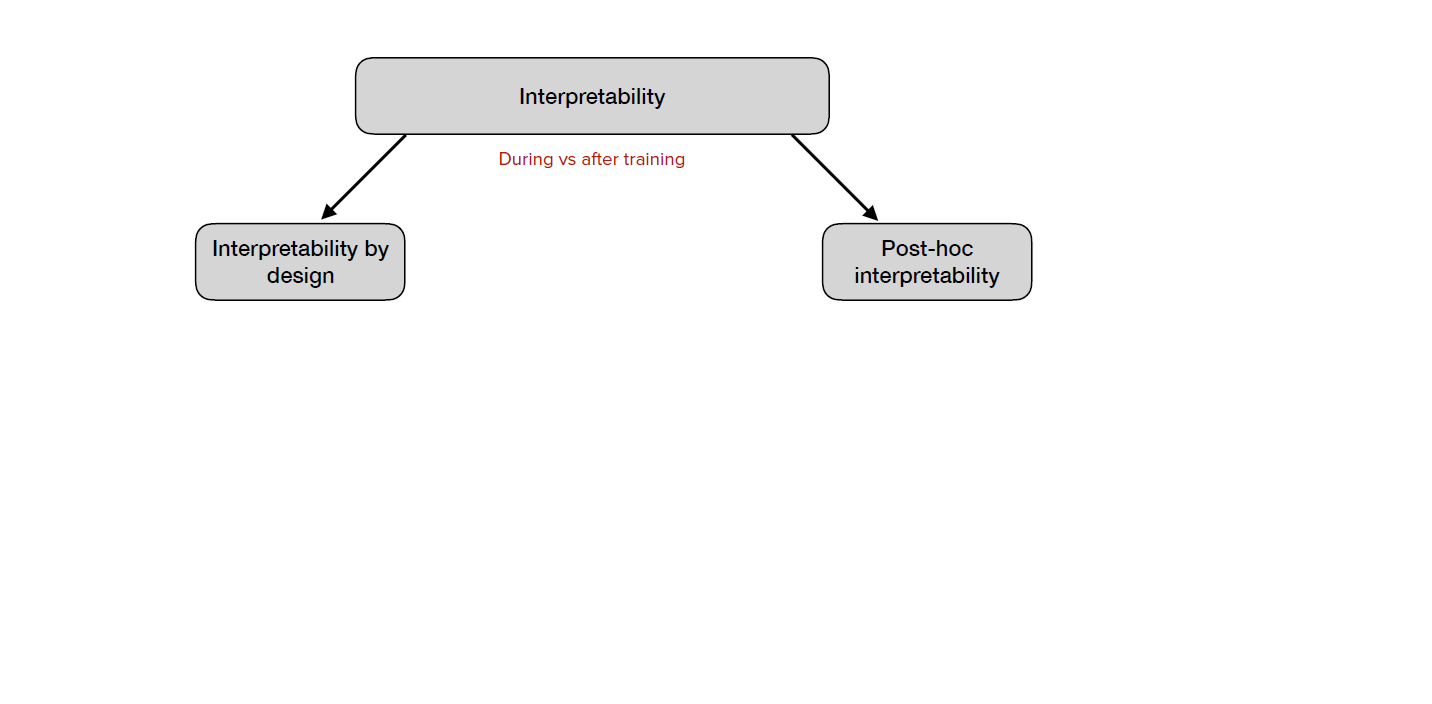
\includegraphics[scale=.4]{baum1}
%\end{figure}
\end{frame}

\begin{frame}[c]{Interpretability landscape in Neural Networks}
%\begin{figure}
    
    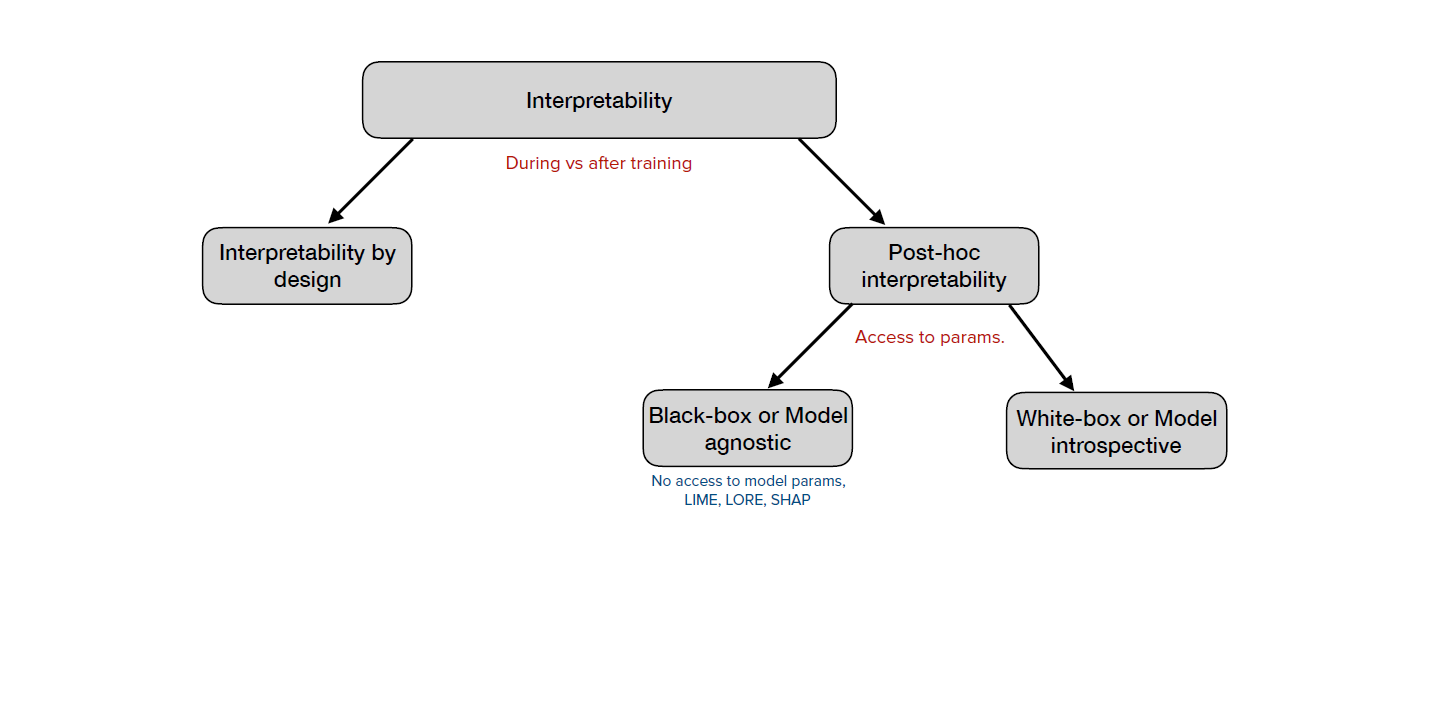
\includegraphics[scale=.4]{baum2}
%\end{figure}
\end{frame}

\begin{frame}[c]{Interpretability landscape in Neural Networks}
%\begin{figure}
    
    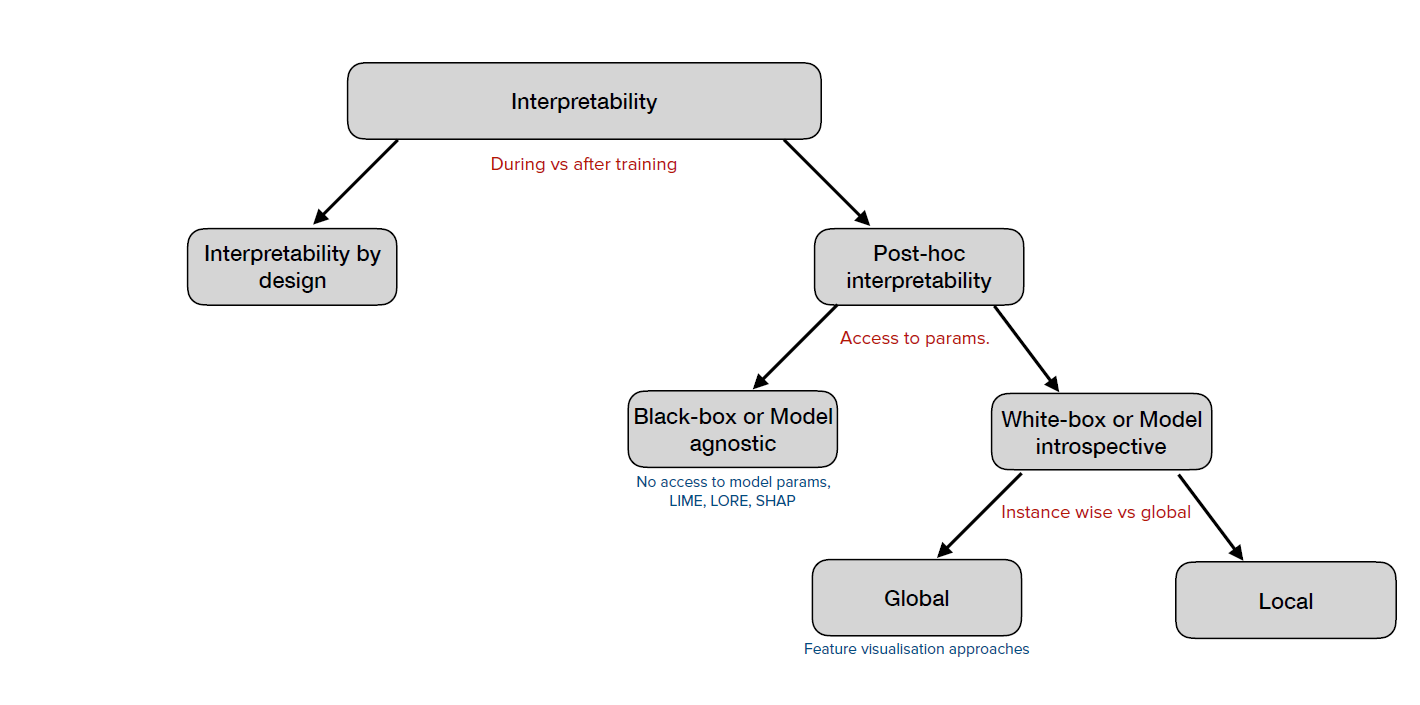
\includegraphics[scale=.4]{baum3}
%\end{figure}
\end{frame}

\begin{frame}[c]{Interpretability landscape in Neural Networks}
%\begin{figure}
   
    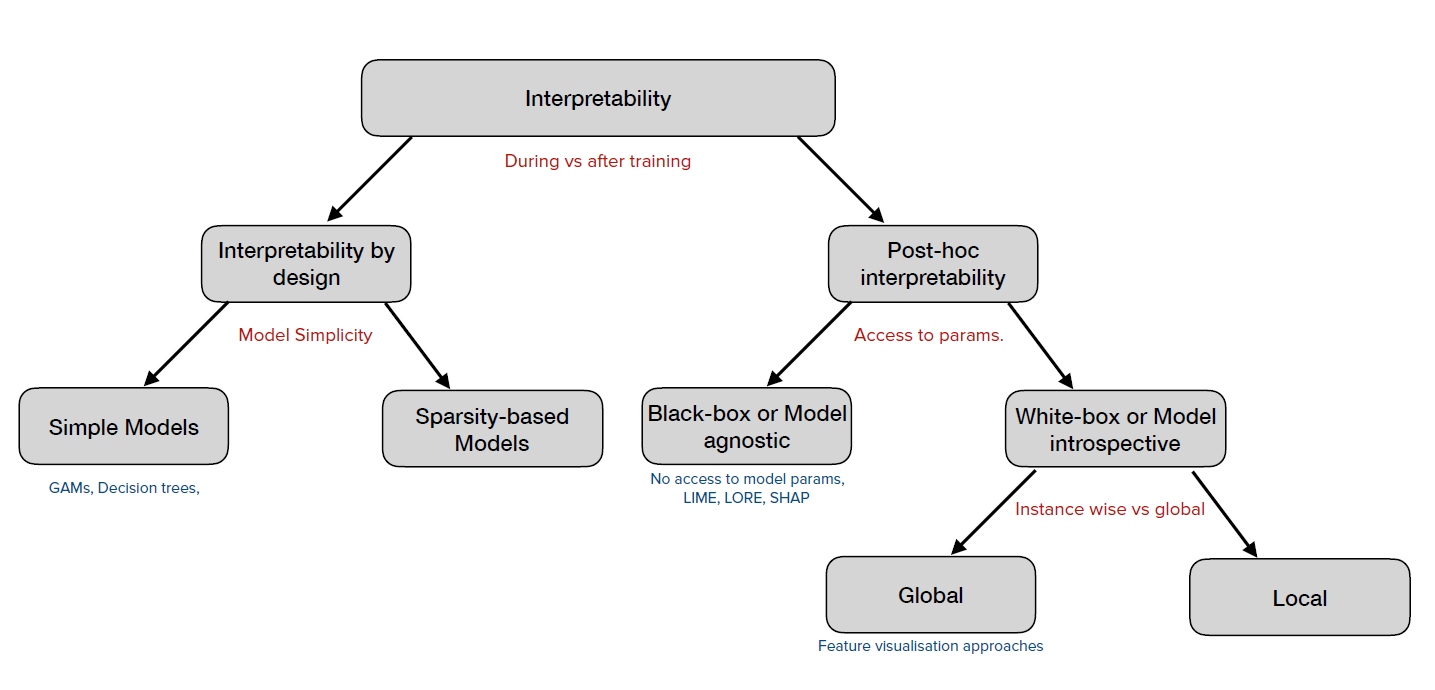
\includegraphics[scale=.4]{baum4}
%\end{figure}
\end{frame}


\begin{frame}[c]{Interpretability landscape in Neural Networks}
%\begin{figure}
    
    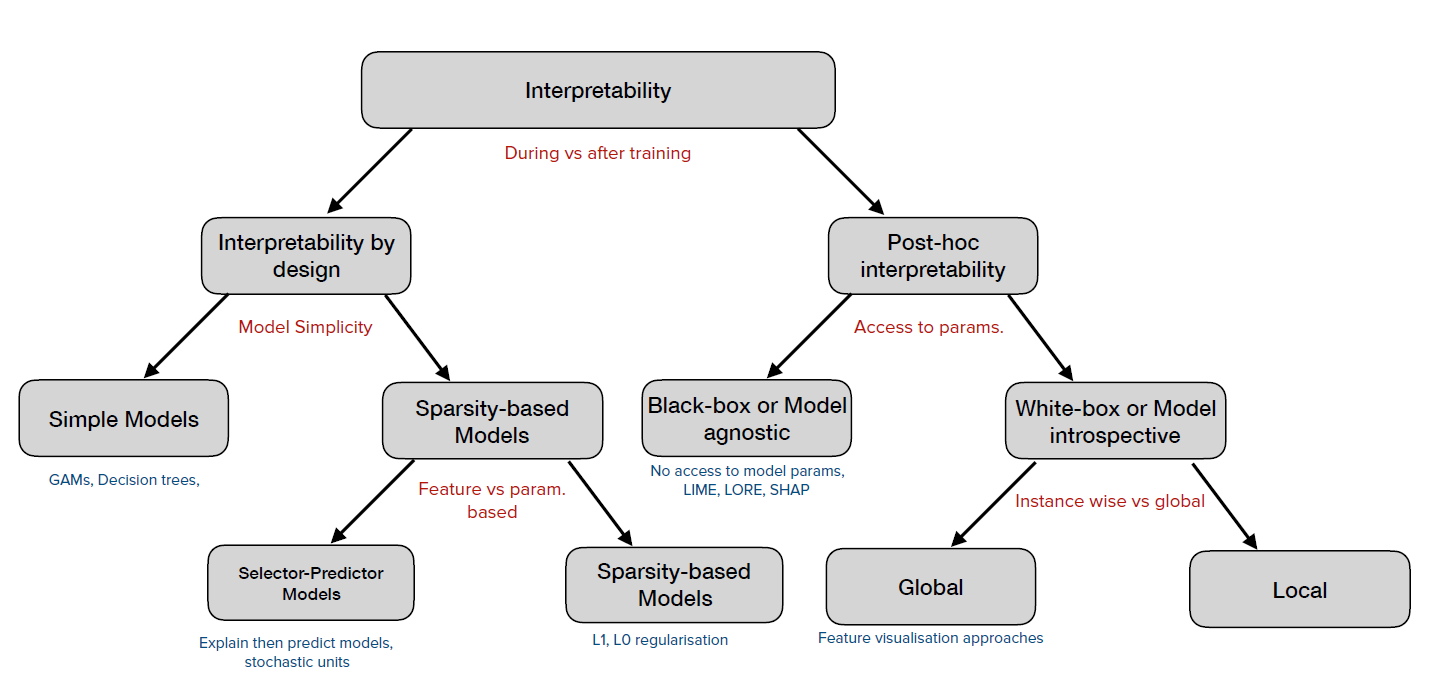
\includegraphics[scale=.4]{baum5}
%\end{figure}
\end{frame}






\begin{frame}[c]{How can we interpret Neural Models ?}
	\begin{itemize}
		\item Feature visualization: Visualizing components of the neural networks
		\begin{itemize}
			\item Activations of neurons
			\item Attention values
			\item Gradient flow
		\end{itemize}
		\item Feature attributions: relevant input features
		\begin{itemize}
			\item Which input features are responsible for the given decision ?
			\item Sensitivity analysis using gradient-based methods
			\item Using black-box methods like LIME, SHAP, etc.
		\end{itemize}
	\end{itemize}
\end{frame}

\begin{frame}[c]{How can we interpret Neural Models ?}

	\begin{figure}
	\centering
\hfill

  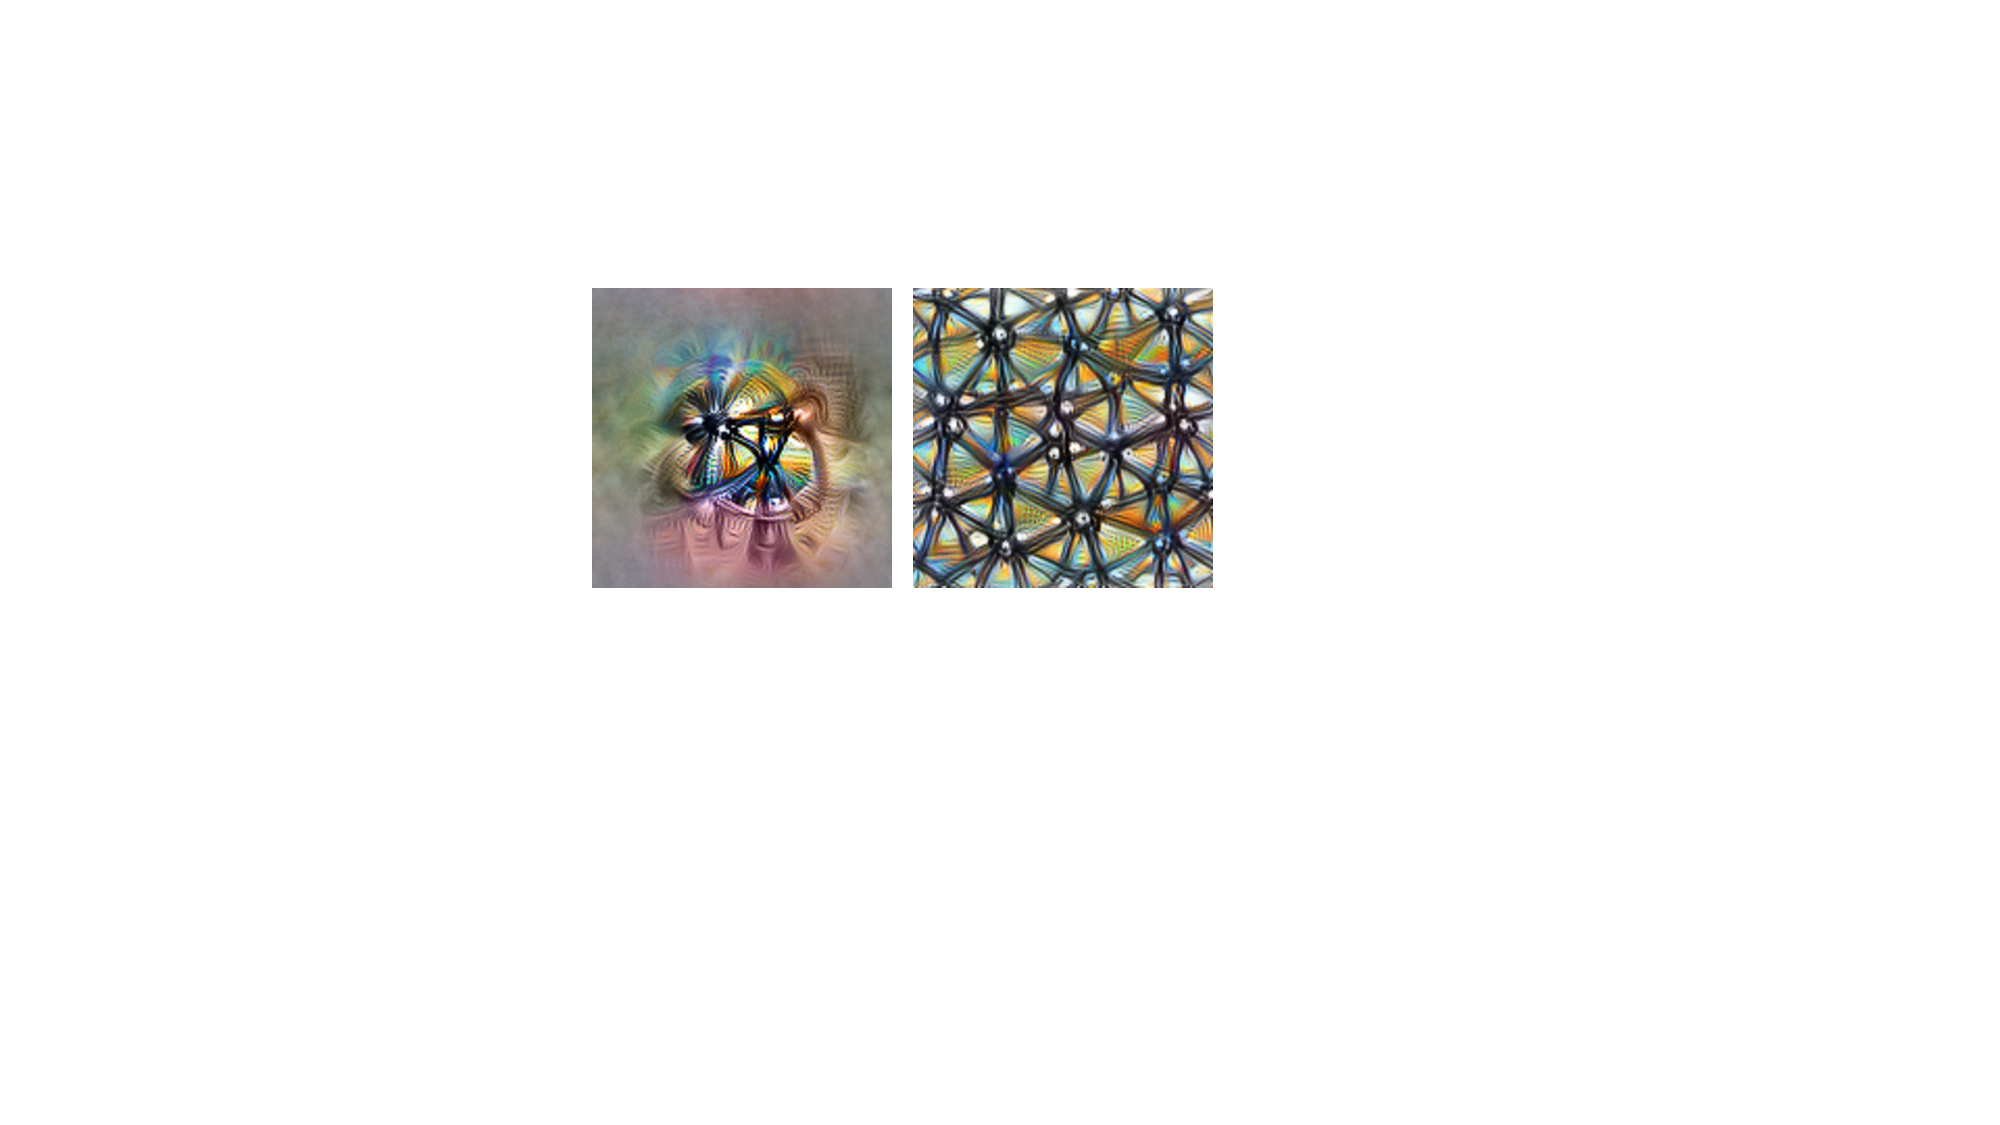
\includegraphics[width=0.6\linewidth]{figure/iml-grad-vis.pdf}
  
  \caption{Feature visualization: Visualizing components of the neural networks}

\end{figure}
\end{frame}


\begin{frame}[c]{How can we interpret Neural Models ?}

\begin{figure}[h]
	\centering
	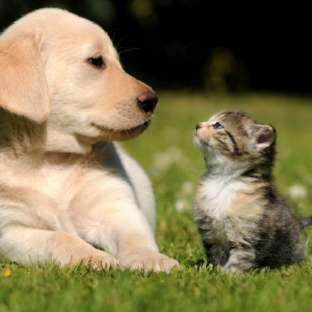
\includegraphics[width=0.3\linewidth]{figure/img145.jpg}
	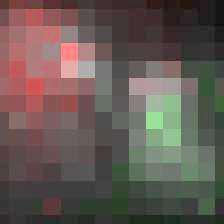
\includegraphics[width=0.3\linewidth]{figure/img149.jpg}
	\caption{Feature attributions: relevant input features}
\end{figure}
\end{frame}

\endlecture
\end{document}